%%%%%%%%%%%%%%%%%%%%%%%%%%% asme2ej.tex %%%%%%%%%%%%%%%%%%%%%%%%%%%%%%%
% Template for producing ASME-format journal articles using LaTeX    %
% Written by   Harry H. Cheng, Professor and Director                %
%              Integration Engineering Laboratory                    %
%              Department of Mechanical and Aeronautical Engineering %
%              University of California                              %
%              Davis, CA 95616                                       %
%              Tel: (530) 752-5020 (office)                          %
%                   (530) 752-1028 (lab)                             %
%              Fax: (530) 752-4158                                   %
%              Email: hhcheng@ucdavis.edu                            %
%              WWW:   http://iel.ucdavis.edu/people/cheng.html       %
%              May 7, 1994                                           %
% Modified: February 16, 2001 by Harry H. Cheng                      %
% Modified: January  01, 2003 by Geoffrey R. Shiflett                %
% Use at your own risk, send complaints to /dev/null                 %
%%%%%%%%%%%%%%%%%%%%%%%%%%%%%%%%%%%%%%%%%%%%%%%%%%%%%%%%%%%%%%%%%%%%%%

%%% use twocolumn and 10pt options with the asme2ej format
\documentclass[twocolumn,10pt]{asme2ej}

\usepackage{graphicx} %% for loading jpg figures
\usepackage{mathtools}
\usepackage{moreverb,url}

%% The class has several options
%  onecolumn/twocolumn - format for one or two columns per page
%  10pt/11pt/12pt - use 10, 11, or 12 point font
%  oneside/twoside - format for oneside/twosided printing
%  final/draft - format for final/draft copy
%  cleanfoot - take out copyright info in footer leave page number
%  cleanhead - take out the conference banner on the title page
%  titlepage/notitlepage - put in titlepage or leave out titlepage
%  
%% The default is oneside, onecolumn, 10pt, final


\title{Experimental Validation for Surface Type Dependency of Ground Effect on Quadrotors}

%%% first author
\author{Alejandro Dena \thanks{j.a.dena-ruiz@cranfield.ac.uk} 
    \affiliation{
        Cranfield University\\
        Centre for Electronic Warfare,\\ Information and Cyber\\
        Defence Academy of the United Kingdom\\
        Shrivenham\\
        SN6~8LA, UK.
    }	
}

%%% second author
%%% remove the following entry for single author papers
%%% add more entries for additional authors
\author{Kenan Ahiska \\
    \affiliation{ 
        Cranfield University\\
        Centre for Electronic Warfare,\\ Information and Cyber\\
        Defence Academy of the United Kingdom\\
        Shrivenham\\
        SN6~8LA, UK.
    }
}

%%% third author
%%% remove the following entry for single author papers
%%% add more entries for additional authors
\author{Prof. Nabil Aouf
    \affiliation{
        City, University of London\\
        Northampton Square\\
        London EC1V 0HB\\
        United Kingdom\\
    }
}


\begin{document}

\maketitle    

%%%%%%%%%%%%%%%%%%%%%%%%%%%%%%%%%%%%%%%%%%%%%%%%%%%%%%%%%%%%%%%%%%%%%%
\begin{abstract}
{\it The ground effect is an aerodynamic phenomena which reduces the induced drag on aircraft and thereby increases its lift-to-drag ratio. In the case of aerial vehicles with propellers, the rotor lift force during hover increases when the vehicle flights close to a surface. This paper presents an empirical analysis of this lift force acting on quadrotors with different propeller sizes and hovering over various surface types. A new mathematical model for ground effect which comprises surface type dependency is proposed and verified experimentally. Modelling error is reduced by 14\% in average compared to the most sophisticated ground effect model available in the literature. A ground effect compensator for quadrotor altitude control is introduced to verify the modelling accuracy of the proposed approach. In terms of altitude tracking errors, a 20-80\% improvement is achieved with the proposed model. Furthermore, it is observed that in average the compensator based on the proposed model reduces the control effort by half compared to that attained with previous models.
}
\end{abstract}

%%%%%%%%%%%%%%%%%%%%%%%%%%%%%%%%%%%%%%%%%%%%%%%%%%%%%%%%%%%%%%%%%%%%%%
% \begin{nomenclature}
% \entry{A}{You may include nomenclature here.}
% \entry{$\alpha$}{There are two arguments for each entry of the nomemclature environment, the symbol and the definition.}
% \end{nomenclature}

% The primary text heading is  boldface and flushed left with the left margin.  The spacing between the  text and the heading is two line spaces.

%%%%%%%%%%%%%%%%%%%%%%%%%%%%%%%%%%%%%%%%%%%%%%%%%%%%%%%%%%%%%%%%%%%%%%
\section{Introduction}

Over the last decade, quadrotors have been one of the most popular Unmanned Aerial Vehicles (UAV), due to their small size and capabilities to hover and reach difficult-to-access areas. Exploration, detection, localisation and surveillance are some of the most common applications for this particular type of UAVs, \cite{Jaimes2008, Lee2017, Alvissalim2012}. Although most of the applications require a stable drone flying at high altitudes, some applications such as landmine detection demand a steady flight and hovering close to the ground. An additional aerodynamic effect due to the proximity to the ground surface or the presence of different objects in close vicinity, namely \textit{the ground effect}, introduces further challenges for the control of the UAV hovering, \cite{Johnson1994}.

For helicopters, the ground effect is perceived as an increase on the lift force during hover due to the interaction of the rotor airflow with the ground surface, \cite{Tanner2015}, \cite{Xin1999}. Analogously to the helicopters, for UAVs with a single rotor, ground effect is defined as a factor increasing the lift force. Nevertheless, the available literature regarding ground effect is substantially limited.

The most accepted ground effect model is based on method of images and potential flow, proposed by Cheeseman and Bennet, \cite{Cheeseman1955}. This model accurately predicts the ground effect for helicopters, and for single rotor UAVs at the altitudes lower than two times of the radius of their propeller.

In addition to models based on method of images, for single-rotor UAVs, Nonaka et al. proposed curve fitting techniques to describe ground effect, \cite{Nonaka2011}. They used empirical data obtained at different altitudes and identified the coefficients of a second order polynomial by curve fitting on the recordings of voltage applied to the rotor as an indicator to the hover thrust. Their model showed the presence of ground effect at heights up to almost five times the radius of the propeller. %The \textit{ground effect} is an aerodynamic phenomena that occurs on the aforementioned conditions.

For the case of multi-rotors, the model should be defined carefully, since the airflow produced by a rotor is influenced by the other rotors. Matus et.al tested the model in \cite{Cheeseman1955} on a nano quadrotor, and they concluded that the desired behavior can not be approximated with this model, \cite{AMVargas2017}. Therefore, the authors altered the model by replacing the fixed rational constant of radius to altitude, with a parameter $k$ which was estimated from the empirical data with curve fitting techniques. In another study, Danjun et al. modified the model in \cite{Cheeseman1955} and added a new term $\rho$ which was estimated from empirical data acquired at different altitudes for their specific quadrotor with propellers of 15 inches diameter, \cite{Danjun2015}. Their results showed that for their quadrotor, the ground effect is perceived up to an altitude of four times the radius of the propeller, as also described in \cite{Powers2013}.

The model in \cite{Cheeseman1955} was also expanded by Sanchez-Cuevas et al.\cite{Sanchez-Cuevas2017}, from a single rotor to a quadrotor by adding a term to be tuned with empirical data to achieve a better ground effect estimate. This model showed that the ground effect for multi-rotors is significant for distances up to five times the propeller radius. In another study, D. Bernard et al. used a second order polynomial and least square estimates for determining the coefficients of the polynomial, to represent the ground effect for a single rotor from its thrust response, using an special test bench, \cite{Bernard2017}. They then extended their method to generalize their model to four rotors.

There is also a very particular study on an unusual type of multirotors: the Draganflyer X8, \cite{Sharf2014}. This UAV is actuated by 8 propellers arranged in 4 coaxial pairs in a cross structure configuration. The authors compared the model in \cite{Cheeseman1955} and their proposed model, which uses curve fitting on a second order polynomial. 

Accurate modeling of ground effect is important for quadrotor control since various studies prove that ground effect has an impact on the stability of the quadrotors. For example, in \cite{Davis2016}, Davis et al. worked on the stability of a quadrotor with canted rotors in a sloped channel and showed that increasing the rotor's cant produces bigger damping, whereas changing the channel slope results in a higher position feedback, which should be taken into consideration in controller design. Furthermore, the impact of ground effect on the roll and pitch stability of a quadrotor as a function of its altitude was studied in frequency domain, by S. Aich et al., in \cite{Aich2014}. 

Ground effect introduces significant issues in control applications, \cite{Bartholomew2015}. In his study, Bartholomew demonstrated a technique to improve flight control of micro aerial vehicles that experience aerodynamic disturbances caused by objects in their flight path. A robust altitude control with ground effect compensation for a small RC helicopter is also proposed in \cite{Nonaka2011}. As an alternative to the altitude measurement, for ground effect compensation, visual feedback can be used to estimate external disturbances on a quadrotor, as in the work of Rayan et al. \cite{Ryan2012}.

In \cite{Nobahari2014}, another model for ground effect is proposed, based in the model founded in \cite{Hayden1976}. The based model in Nobahari's work, is an extension of the model proposed by Hayden, considering the addition of the distance from the quadrotor's center of mass to the propellers $R_{eq}$. This study is oriented to the ground effect compensation for landing operations and the altitude state estimation. 

The limited literature on ground effect hardly  approximates it as a function of altitude for different rotor sizes. It is also observed that surface type is not even considered as a factor in ground effect modelling. In this study, we demonstrated though extensive experiments (at 13 different altitudes, with 3 different rotor sizes and over 4 different surface types) that ground effect depends on surface type as well. In this paper, this phenomena is introduced and a surface type dependent ground effect model is proposed. According to the analysis on experimental data, it is observed that the proposed model generates smaller modelling errors compared to the other models available in the literature. Furthermore, a ground effect compensated controller design is implemented and the improvement in the reference tracking performance. 

The structure of this paper is as follows: in Section II, a mathematical model for a quadrotor is introduced. Section III explains the ground effect phenomena and the models available in the literature. In Section IV, our experimental setup is demonstrated and the accuracies of the available ground effect models are assessed in comparisons with the experimental data. In Section V, surface type dependent ground effect model is proposed  and the improvement achieved in the modelling accuracy is demonstrated. Finally, section VI presents the controller design for quadrotors including the ground effect compensation and the reduction in the controller effort are presented as further verification tests for the proposed model.

\section{Quadrotor Model}\label{quad_model_section}
A mathematical model for quadrotors is defined based on Newton-Euler equations, \cite{GarciaCarrillo2013} \cite{Bouabdallah2005}. In order to eliminate unnecessary complexity, the quadrotor is assumed to be symmetric and rigid. The reference frames and key variables are presented in Fig. \ref{quad_frames}, where $\mathcal{F}_{I}$ represents the inertial frame fixed at a point on the ground and with its $z$ axis pointing upwards, the $x$ and $y$ axes can be chosen following the right hand convention. $\mathcal{F}_{B}$ represents the body frame, with its coordinate axes aligned with $\mathcal{F}_{I}$ and its origin is at the center of gravity of the quadrotor, which is assumed to coincide with its geometric centre. Also each propeller have a rotational velocity $\Omega_{i}$ with $i=1:4$, $\Omega_{1}$ and $\Omega_{2}$ are in counter-clockwise direction, whilst $\Omega_{3}$ and $\Omega_{4}$ are in the clockwise direction.

Using Newton's laws of mechanics and Euler's dynamics, the model consists of six equations for the system dynamics and four equations to describe the inputs, as shown in Eqn.\eqref{model_1}-\eqref{model_6}, where $m$ is the total quadrotor mass, Eqn.\eqref{model_1} - \eqref{model_3} describe the linear accelerations defined in the $\mathcal{F}_{I}$, while Eqn.\eqref{model_4} - \eqref{model_6} represent the angular accelerations about the centre of gravity of the vehicle in $\mathcal{F}_{B}$. $l$ corresponds to the arm length holding the propeller, $\phi$, $\theta$ and $\psi$ represent the Euler angles. $I_{xx}$, $I_{yy}$ and $I_{zz}$ are the body inertial components, and $J_{r}$ and $\Omega$ are the rotor inertia and rotor speed, respectively. $U_{1}$, $U_{2}$, $U_{3}$ and $U_{4}$ represent the control inputs, as well as total force provided by the four rotors, and the torques in each of the rotation axis. These last four variables will be the system inputs, and are related to the propeller speeds as described in Eqn. \eqref{model_7}-\eqref{model_11}. 

%%%%%%%%%%%%%%%% begin figure %%%%%%%%%%%%%%%%%%%
\begin{figure}[t]
    \begin{center}
    \setlength{\unitlength}{0.012500in}%
    \includegraphics[width=8.5cm, height=6cm]{Images/quad_frames.png}
    \end{center}
    \caption{Body and Inertial frames}
    \label{quad_frames} 
\end{figure}
%%%%%%%%%%%%%%%% end figure %%%%%%%%%%%%%%%%%%% 

\begin{align}
    \ddot{X}      &= (\cos\phi\sin\theta\cos\psi + \sin\phi\sin\psi)\frac{1}{m}U_{1} \label{model_1}\\
    \ddot{Y}      &= (\cos\phi\sin\theta\sin\psi - \sin\phi\cos\psi)\frac{1}{m}U_{1}  \label{model_2}\\
    \ddot{Z}      &= (\cos\phi\cos\theta)\frac{1}{m}U_{1} - g \label{model_3}\\ 
    \ddot{\phi}   &= \dot{\theta}\dot{\psi}(\frac{I_{yy}-I_{zz}}{I_{xx}})-\frac{J_{r}}{I_{xx}}\dot{\theta}\Omega+\frac{l}{I_{xx}}U_{2}\label{model_4}\\
    \ddot{\theta} &= \dot{\phi}\dot{\psi}(\frac{I_{zz}-I_{xx}}{I_{yy}})+\frac{J_{r}}{I_{yy}}\dot{\phi}\Omega+\frac{l}{I_{yy}}U_{3} \label{model_5}\\
    \ddot{\psi}   &= \dot{\phi}\dot{\theta}(\frac{I_{xx}-I_{yy}}{I_{zz}})+\frac{U_{4}}{I_{zz}} \label{model_6}\\
    U_{1}  &= b_{f}(\Omega_{1}^{2} + \Omega_{2}^{2} + \Omega_{3}^{2} + \Omega_{4}^{2}) \label{model_7}\\ 
    U_{2}  &= b_{f}l(\Omega_{2}^{2} + \Omega_{4}^{2}) \label{model_8} \\
    U_{3}  &= b_{f}l(\Omega_{3}^{2} + \Omega_{1}^{2}) \label{model_9} \\
    U_{4}  &= d_{f}(\Omega_{1}^{2} + \Omega_{3}^{2} - \Omega_{2}^{2} - \Omega_{4}^{2}) \label{model_10} \\
    \Omega &= \Omega_{1}^{2} + \Omega_{3}^{2} + \Omega_{2}^{2} + \Omega_{4}^{2} \label{model_11}
\end{align}

where $b_{f}$ is positive constant which denotes the thrust factor of a propeller, $l$ is the distance from one of the rotors to the center of gravity and $d_{f}$ is the drag factor.

\section{Defining The Ground Effect} 
It is well known that aerial vehicles with rotors tend to experience some aerodynamic effects as they fly close to surfaces or objects. The aerodynamic effect produced by the interaction between the ground surface and the aerial vehicles is called \textit{ground effect} and it alters the total vehicle thrust.

For helicopters, this phenomena increases the total thrust when hovering close to the ground, due to the air pressure accumulating between the rotor propeller and the ground surface. The widely used ground effect model is based on potential flow and the method of images, proposed by Cheeseman \& Bennet, \cite{Cheeseman1955}. In this model, the ground effect is represented in the form of a thrust force as a function of the propeller radius and the distance from the propeller to the ground surface, as given in Eqn.\eqref{chessman}. Here $T_{IGE}$ and ${T_{OGE}}$ refer to the thrust force while hovering in the ground effect and out of this region, respectively. $R$ is the propeller radius and $z$ is the altitude of the vehicle.

\begin{equation}
\frac{T_{IGE}}{T_{OGE}} = \frac{1}{1-(\frac{R}{4z})^{2}} \label{chessman}
\end{equation}

For the case of multirotors, the ground effect becomes complex due to the aerodynamic interaction between a rotor and its neighboring rotors. For multirotors, Danjun et.al proposed a ground effect model based on Eqn.\eqref{chessman} which modifies this equation and adds a $\rho$ coefficient, estimated from the experimental data at different heights using a least square approximation, \cite{Danjun2015}. As given in Eqn.\eqref{danjun}, this model was applied to a quadrotor, and the results prove the existence of ground effect up to altitudes $z/R = 4$.

\begin{equation}
\frac{T_{IGE}}{T_{OGE}} = 1-\rho(\frac{R}{4z)^{2}}  \label{danjun}
\end{equation}

Another extension of the model in Eqn.\eqref{chessman} for multirotors uses potential flow and the method of images applied to a quadrotor \cite{Sanchez-Cuevas2017}, is presented in Eqn.\eqref{sanchez-cuevas_1}. Here $d$ represents the separation from each rotor axis to its adjacent rotor axes, R is the radius of the rotor and $z$ is the vertical distance of the rotor to the ground.

\begin{align}
  \frac{T_{IGE}}{T_{OGE}} = \frac{1}{\splitfrac{1 - (\frac{R}{4z})^{2} - R^{2}(\frac{z}{\sqrt{(d^{2}+4z^{2})^{3}}})} 
  {- (\frac{R^{2}}{2})(\frac{z}{\sqrt{(2d^{2}+4z^{2})^{3}}})}}  \label{sanchez-cuevas_1} 
\end{align}

Using empirical measurements, it is observed that the model in Eqn.\eqref{sanchez-cuevas_1} gives a considerable accurate representation of the ground effect for quadrotors. Nevertheless, some residuals between the model and the empirical data remain, \cite{Sanchez-Cuevas2017}. In the most recent improvement in ground effect model, a new parameter $b$ that represents the distance between the two opposite rotor axes (diagonal) was introduced to the model, and an additional term to compensate this difference was added to Eqn.\eqref{sanchez-cuevas_1}. This model, given in Eqn.\eqref{sanchez-cuevas_2}, includes the so-called \textit{"the body lift coefficient"} represented by the $k_{b}$, a positive term that can be identified by fitting the model to the empirical data.

\begin{align}
  \frac{T_{IGE}}{T_{OGE}} = \frac{1}{\splitfrac{1 - (\frac{R}{4z})^{2} - R^{2}(\frac{z}{\sqrt{(d^{2}+4z^{2})^{3}}})} {- (\frac{R^{2}}{2})(\frac{z}{\sqrt{(2d^{2}+4z^{2})^{3}}}) - 2R^{2}(\frac{z}{\sqrt{(b^{2}+4z^{2})^{3}}}k_{b})}}  \label{sanchez-cuevas_2}
\end{align}

\section{Initial experimental analysis and assessment}
The modeling performances of the aforementioned proposals are experimentally evaluated. However, there is no standard experimental setup for testing the ground effect. In \cite{Sanchez-Cuevas2017}, the experiments were conducted on a special test bench, where the quadrotor was placed at different heights and force sensors were used to measure the thrust for each rotor separately. On the other hand, in \cite{Bernard2017}, as an experimental setup, the quadrotor was rigidly attached to a testbed that allows changes in the height from the ground, and a 6 DoF load cell was used to measure the total force at each height. Note that both of these experimental setups constrain the motion of UAV and hence they lack accuracy in modeling the ground effect during a free flight.

\subsection{Experimental setup}
In this study, the experiments are conducted in a controlled environment in our laboratory. The environment is wind-free and also equipped with precise position measuring tools such as the OptiTrack system \cite{Optitrack}, allowing to execute experiments whit the quadrotor in free flight and with no attachments. Fig. \ref{Arena} shows the layout of the used arena. The box area in the middle is changed during tests with different surface types.

\begin{figure}[t]
  \begin{center}
  \setlength{\unitlength}{0.012500in}%
  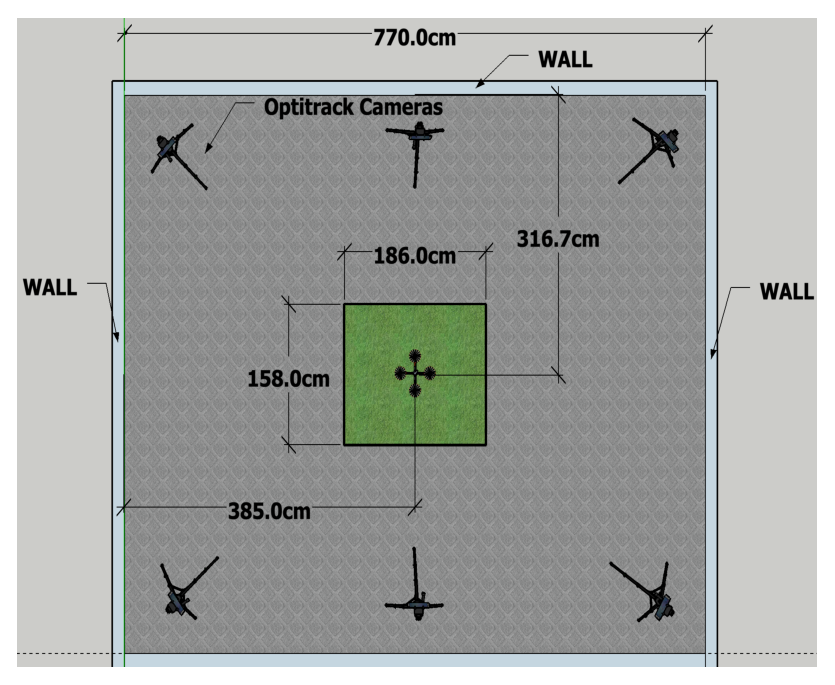
\includegraphics[width=8.5cm, height=6cm]{Images/arena.eps}
  \end{center}
  \caption{Arena where experiments were performed}
  \label{Arena}
\end{figure}

The distance from the ground to the ceiling is 3 m. Only 3 walls are shown on the schematic in Fig. \ref{Arena}, and the downside wall in the figure is 5 m away. Note that the maximum altitude during the experiments is 1 m; hence, effects due to the ceiling and the downside wall are neglected. 

The Pelican quadrotor from AscTec (Ascending Technologies)\cite{AscTec} is chosen as the prototype to develop the experiments. Its physical structure is made of carbon fibre, and its well distributed sensors and components make it a reliable platform for research purposes. This quadrotor offers plenty of space and various interfaces for individual components and payloads, see Fig. \ref{Pelican}.

\begin{figure}[t]
    \begin{center}
        \setlength{\unitlength}{0.012500in}%
        \includegraphics[width=8.5cm, height=6cm]{Images/Pelican.eps}
    \end{center}
    \caption{Quadrotor AscTec Pelican with autopilot and mastermind}
    \label{Pelican}
\end{figure}

Detailed information regarding the quadrotor setup can be found in our previous work, in \cite{DenaRuiz2017}. Three different size of propellers as shown in Fig. \ref{props}, are used during the experiments to understand the dependency of the ground effect on different propeller sizes. Table \ref{props_params} shows the related parameters for the propellers that are used in experiments; their thrust coefficients and the total drone mass for each size. The Pitch angle or blade pitch refers to the turning angle of attack of the blades of a propeller or helicopter rotor.

\begin{figure}[t]
    \begin{center}
        \setlength{\unitlength}{0.012500in}%
        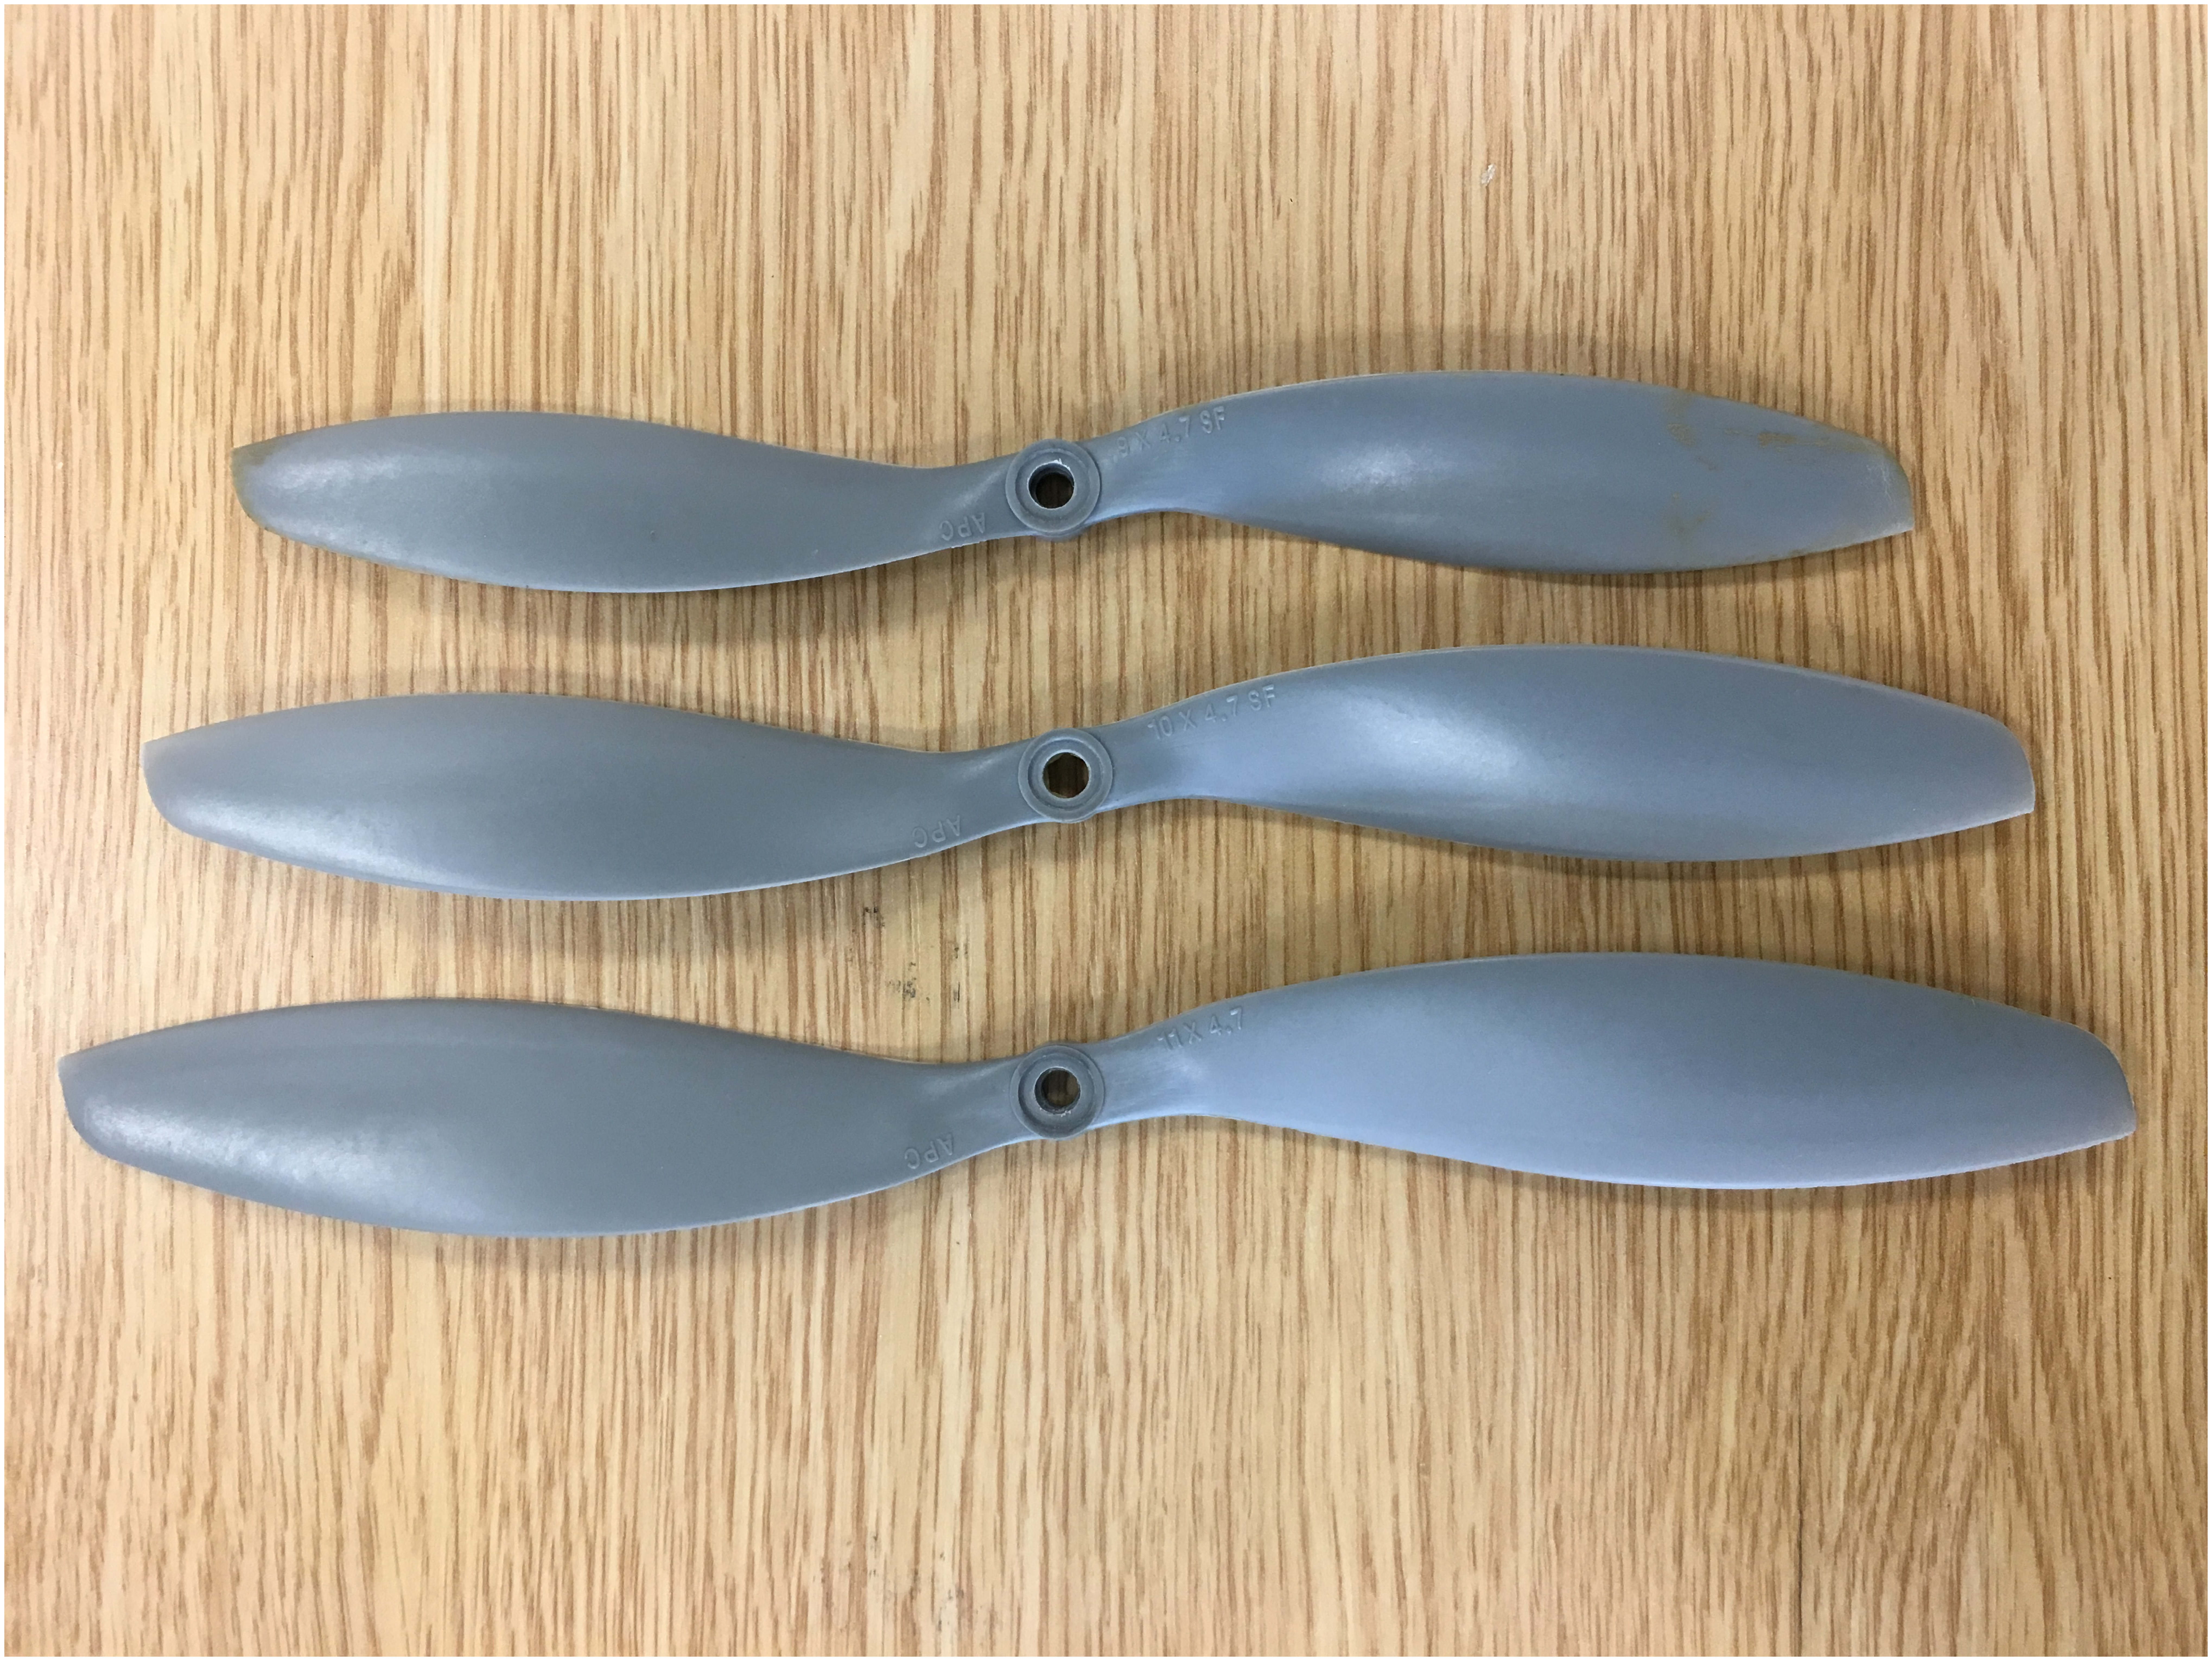
\includegraphics[width=8.5cm, height=6cm]{Images/props.eps}
    \end{center}
    \caption{Three different propellers used in the experiments}
    \label{props}
\end{figure} 

%%%%%%%%%%%%%%% begin table   %%%%%%%%%%%%%%%%%%%%%%%%%%
\begin{table}[t]
    \small
    \caption{Propeller characteristics and their thrust coefficients}
    \begin{center}
    \label{props_params}
    \scalebox{0.8}{
    \begin{tabular}{c c c c c}
    & & & &\\ % put some space after the caption
    \hline
    Propeller & Radius(\textit{inch}) & Pitch(\textit{inch}) & Thrust Coef($b_{f}$) & Quadrotor's \\
    &                       &                      &                  & Mass($kg$)\\
    \hline
    APC 0947 & 4.5 & 4.7 & $8.20\times10^{-6}$ & 1.501\\
    APC 1047 & 5.0 & 4.7 & $1.49\times10^{-5}$ & 1.518\\
    APC 1147 & 5.5 & 4.7 & $1.81\times10^{-5}$ & 1.524\\
    \hline
    \end{tabular}}
    \end{center}
\end{table}
%%%%%%%%%%%%%%%% end table %%%%%%%%%%%%%%%%%%% 

The communication framework of the experimental setup is presented by the block diagram in Fig. \ref{comm_block_diagram}. All the communications between the ground station computer and the quadrotor are preformed through a WiFi network using ROS (Robot Operating System). The quadrotor position is obtained from Optitrack \cite{Optitrack} at 120 Hz. Individual ROS packages running on the quadrotor's onboard computer and the ground station perform the full control of the UAV and save the real time data during flight.

\begin{figure}[t]
    \begin{center}
        \setlength{\unitlength}{0.012500in}%
        \includegraphics[width=8.5cm, height=4cm]{Images/block_diagram.eps}
    \end{center}
    \caption{Communication block diagram}
    \label{comm_block_diagram}
\end{figure}

A total of four surface types are selected to perform the experiments: turf, dry soil, irregular dry soil, and dirt as shown in Fig. \ref{surface_types}.

\begin{figure}[t]
    \begin{center}
        \setlength{\unitlength}{0.012500in}%
        \includegraphics[width=8.5cm, height=6cm]{Images/surface_types.eps}
    \end{center}
    \caption{Four surface types: dirt on the top left, dry soil on the top right, irregular dry soil on the bottom left, and turf on the bottom right}
    \label{surface_types}
\end{figure}

The experiments are performed by hovering the quadrotor at 13 different heights: 1.0, 0.9, 0.8, 0.7, 0.6, 0.55, 0.5, 0.45, 0.4, 0.35, 0.3, 0.25, and 0.21 m. Here, the height represent the distance from the propellers to the ground surface, having the minimum value of 21 cm when the quadrotor is on the surface. An average of 500 samples (7 seconds) for each system variable are recorded at each height in real-tme.

In order to get an estimation of the ground effect force, it is assumed that this force is proportional to the total force ($f_{T}$). Solving equations Eqn.\eqref{chessman} to Eqn.\eqref{sanchez-cuevas_2} for $T_{IGE}$ and adding this term to Eqn.\eqref{model_3}, yields to Eqn.\eqref{accZ_GE} and Eqn.\eqref{ge_force}.

\begin{align}
  \ddot{Z} &= (\cos\phi\cos\theta)\frac{1}{m}f_{T}T_{IGE} - g \label{accZ_GE}\\
  T_{IGE}       &= \frac{m(\ddot{Z} + g)}{\cos\phi\cos\theta f_{T}} \label{ge_force}
\end{align}

\subsection{Experimental comparison of the available ground effect models}
In this section, the modelling performance of the available ground effect models are compared against the experimental data. For future reference the models Eqn.\eqref{chessman}, Eqn.\eqref{danjun}, Eqn.\eqref{sanchez-cuevas_1} and Eqn.\eqref{sanchez-cuevas_2} are named as M1, M2, M3, and M4, respectively. Also, $z$ has been defined in section \ref{quad_model_section} as the quadrotor altitude, for the following experiments, $z$ will be considered as the vertical distance from the ground to the rotor propellers. Experimental data for three propeller sizes over four different surface types are collected, and these twelve data sets are employed in this comparison. Note that models M2 and M4 require estimation of the coefficients $\rho$ and $k_{b}$ respectively. These values are calculated by non-linear curve fitting to the experimental data as $\rho = 3.6490$ and $k_{b} = 0.4509$.

\begin{figure}[t]
    \begin{center}
        \setlength{\unitlength}{0.012500in}%
        \includegraphics[width=8.5cm, height=7cm]{Images/r1sx.png}
    \end{center}
  \caption{Comparison of the four existent models vs experimental data from the four surfaces with R = 0.1143 m}
  \label{r1sx_plot}
\end{figure}

\begin{figure}[t]
    \begin{center}
        \setlength{\unitlength}{0.012500in}%
        \includegraphics[width=8.5cm, height=7cm]{Images/r2sx.png}
    \end{center}
  \caption{Comparison of the four existent models vs experimental data from the four surfaces with R = 0.127 m}
  \label{r2sx_plot}
\end{figure}

\begin{figure}[t]
    \begin{center}
        \setlength{\unitlength}{0.012500in}%
        \includegraphics[width=8.5cm, height=7cm]{Images/r3sx.png}
    \end{center}
  \caption{Comparison of the four existent models vs experimental data from the four surfaces with R = 0.1397 m}
  \label{r3sx_plot}
\end{figure}

\begin{figure}[t]
    \begin{center}
        \setlength{\unitlength}{0.012500in}%
        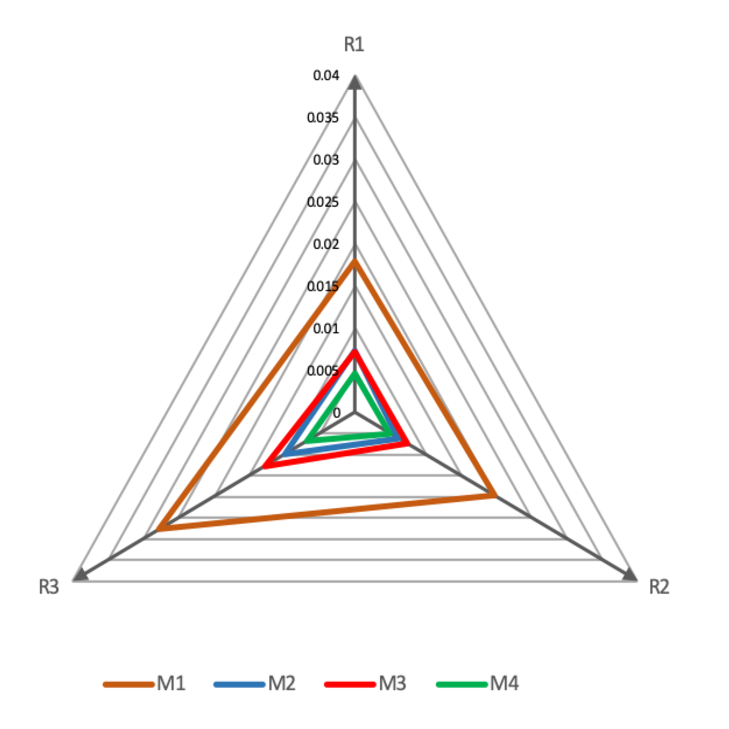
\includegraphics[width=8.5cm, height=8cm]{Images/errors_triangles.eps}
    \end{center}
  \caption{Error comparison between the existent models and the propeller sizes}
  \label{error_comp_r123}
\end{figure}

\begin{table}[!ht]
  \small\sf\centering
  \caption{Errors between the existent models and propeller sizes.}
  \scalebox{0.9}{
  \begin{tabular}{c c c c c}
    & & & &\\ % put some space after the caption
    \hline
    Radii/Model  & M1 & M2 & M3 & M4\\
    \hline
    R1 & 0.017958 & 0.007388	& 0.007244	& 0.004586\\
    R2 & 0.019702 & 0.006084	& 0.007411	& 0.004908\\
    R3 & 0.027704 & 0.009941	& 0.01283	  & 0.006845\\
    \hline
  \end{tabular}}
  \label{props_errors}
\end{table}

Fig. \ref{r1sx_plot}, Fig. \ref{r2sx_plot} and Fig. \ref{r3sx_plot} and Table \ref{props_errors} show the ratio performance $T_{IGE}/T_{OGE}$ against $z/R$, which denotes the distance from the ground to the rotor propellers in terms of the propeller's radii size. The bars on the experimental data indicate the standard deviations of the samples from their mean values. The modelling error in Eqn.\eqref{errors_} is calculated as the absolute sum of the distances between the model prediction and the mean of the experimental data ($\mu_{data}$), at a certain height index $n$ and for the total number of points per height $n$, $d_{np}(n)$. It is observed that M4 exhibits the smallest error among the different models in the literature. Hence, M4 will be used as the reference model for the rest of this paper.

\begin{align}
  \mu_{error} &=  M4(n) - \mu_{data}(n) \label{error_mean} \\ 
  error &= \frac{ \sum_{n=1}^{n=13} d_{np}(n) \mu_{error}(n) }{\sum d_{np}(n)} \label{errors_}
\end{align}

\section{Surface dependent ground effect model}
In this section, surface dependency of the ground effect is investigated. M4 is compared against the experimental data for each surface types separately in Fig. \ref{r1_sx_c_plot}, Fig. \ref{r2_sx_c_plot} and Fig. \ref{r3_sx_c_plot}. Fig. \ref{r1_sx_c_plot} shows this comparison for $R=0.1143$ m, and it is observed that M4 fits the samples for the dry soil surface best with an error of 0.003175 m, but the error starts increasing significantly for the other surface types. Fig. \ref{r2_sx_c_plot} and Fig. \ref{r3_sx_c_plot} show results for other two propeller radii. The curves show that experimental data for different surfaces spread from each other as the radius decreases. The error values are given in Table \ref{props_surface_m4_errors} and Figure \ref{error_comp_r123}.

\begin{figure}[t]
  \begin{center}
  \setlength{\unitlength}{0.012500in}%
  \includegraphics[width=8.5cm, height=7cm]{Images/r1_surface_comp.png}
  \caption{Comparison of M4 vs experimental data from each surface, using R = 0.1143 m}
  \end{center}
  \label{r1_sx_c_plot}
\end{figure}

\begin{figure}[t]
  \begin{center}
  \setlength{\unitlength}{0.012500in}%
  \includegraphics[width=8.5cm, height=7cm]{Images/r2_surface_comp.png}
  \caption{Comparison of M4 vs experimental data from each surface, using R = 0.127 m}
  \end{center}
  \label{r2_sx_c_plot}
\end{figure}

\begin{figure}[t]
  \begin{center}
  \setlength{\unitlength}{0.012500in}%
  \includegraphics[width=8.5cm, height=7cm]{Images/r3_surface_comp.png}
  \caption{Comparison of M4 vs experimental data from each surface, using R = 0.1397 m}
  \end{center}
  \label{r3_sx_c_plot}
\end{figure}

\begin{table}[!b]
  \small\sf\centering
  \caption{Error comparison between M4 and the data samples for each surface type for the 3 propeller radii.}
  \scalebox{0.8}{
  \begin{tabular}{c c c c}
   & & &\\ % put some space after the caption
  \hline
  Surface & R1 (0.1143 m) & R2 (0.127 m) & R3 (0.1397 m) \\
  \hline
  Turf               & 0.009234          & \textbf{0.004585} & 0.009845\\
  Dirt               & 0.006337          & 0.007250          & 0.006478\\
  Irregular Dry Soil & 0.003521          & 0.008313          & 0.006355\\
  Dry Soil           & \textbf{0.003175} & 0.005870          & \textbf{0.005729}\\
  \hline
  \end{tabular}}
  \label{props_surface_m4_errors}
\end{table}

Based on Fig. \ref{r1_sx_c_plot}, Fig. \ref{r2_sx_c_plot} and Fig. \ref{r3_sx_c_plot}, it is evident that the modelling assumption of M4 cannot be valid for different surface types. Hence, an improvement on M4 is necessary to handle different surface types. In this paper, we propose the following innovative model, PM, for ground effect:

\begin{align}
  \frac{T_{IGE}}{T_{OGE}} = \frac{1}{\splitfrac{1 - (\frac{R}{4z})^{2} - R^{2}(\frac{z}{\sqrt{(d^{2}+4z^{2})^{3}}})} {\splitfrac{- (\frac{R^{2}}{2})(\frac{z}{\sqrt{(2d^{2}+4z^{2})^{3}}}) - 2R^{2}(\frac{z}{\sqrt{(b^{2}+4z^{2})^{3}}}k_{b})}{- 2R^{2}(\frac{z}{\sqrt{(b^{2}+4z^{2})^{3}}}k_{s})}}}  \label{sanchez-cuevas_3}
\end{align}

In this equation, in addition to the body lift coefficient $k_{b}$, introduced in Eqn.\eqref{sanchez-cuevas_2}, an empirical surface type dependent lift coefficient $k_{s}$ is considered, which is a positive value. Next to this, the new term uses the velocity of the air at the central point of the body as implemented by \cite{Sanchez-Cuevas2017} in Eqn.\eqref{sanchez-cuevas_2}.
The ground effect results for R=0.1143m, as an example, are shown in Fig. \ref{rxsx_ind_kb}. It is observed that the modelling error is dramatically reduced. For all surface types and propeller radii, modelling errors of M4 and PM are presented in Table \ref{props_surface_PM_errors}. The results show that the modelling errors can be reduced by at least 1.60\%, in average by 13.7\% and up to 56.82\% with the proposed model.

\begin{figure*}[t]
  \begin{center}
  \setlength{\unitlength}{0.012500in}%
  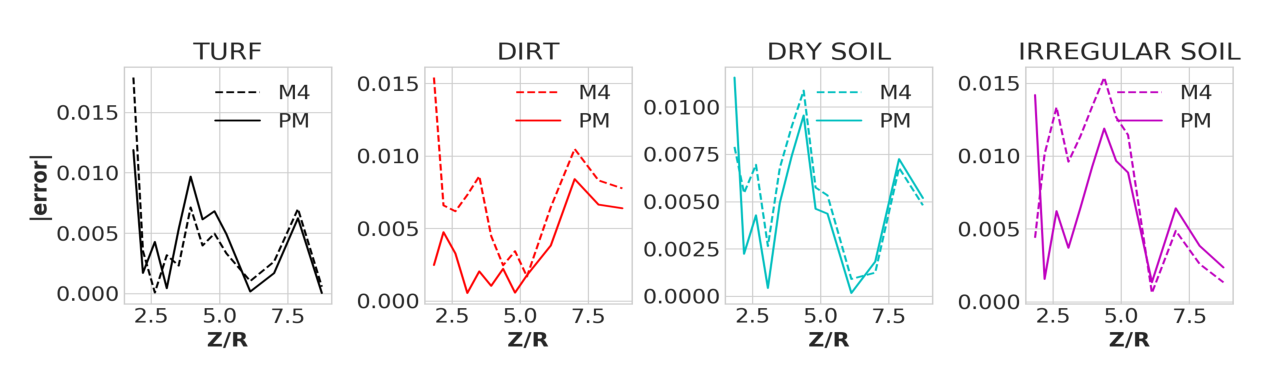
\includegraphics[width=17cm, height=5cm]{Images/errors.eps}
  \end{center}
  \caption{Errors between the mean samples for individual surfaces using M4 and PM, using propeller size R = 0.1143 m, dashed line is M4 and solid line is PM}
  \label{rxsx_ind_kb}
\end{figure*}

\begin{table}
  \small\sf\centering
  \caption{comparison between modelling errors of M4 and PM for different surface types and propeller radii.}
  \scalebox{1.0}{
  \begin{tabular}{c c c c}
    & & &\\ % put some space after the caption
    \hline
    Surface type, radius  & error M4  & error PM  &$\eta$ (\%)\\
    \hline
    Turf, R1              & 0.004585  & 0.004492  &  2.02\\
    Dirt, R1              & 0.007250  & 0.003130  & \textbf{56.82}\\
    Irregular Soil, R1    & 0.005870  & 0.005153  & 12.21\\
    Dry Soil, R1          & 0.008313  & 0.006831  & 17.82\\
    Turf, R2              & 0.009234  & 0.007046  & \textbf{23.69}\\
    Dirt, R2              & 0.006337  & 0.005968  &  5.82\\
    Irregular Soil, R2    & 0.003175  & 0.003226  &  1.60\\
    Dry Soil, R2          & 0.003521  & 0.003007  & 14.59\\
    Turf, R3              & 0.009845  & 0.009488  &  3.62\\
    Dirt, R3              & 0.006478  & 0.006329  &  2.30\\
    Irregular Soil, R3    & 0.006355  & 0.005815  &  8.49\\
    Dry Soil, R3          & 0.005729  & 0.004846  & 15.41\\
    \hline
  \end{tabular}}
  \label{props_surface_PM_errors}
\end{table}

\section{Altitude Control with Ground Effect Compensation} \label{exp_resutls}
The main advantages of quadrotors are their capability of hovering and vertical takeoff and landing. In order to perform these special maneuvers, the altitude control algorithm plays a crucial role. Several control algorithms have been proposed in the literature, from linear to non-linear schemes, \cite{Wicaksono2017, Abci2017, Carrillo2012, Lee2012}.

In this study, to keep the focus on ground effect, altitude controller is selected as a PD controller, the derivation and the performance of this controller can be found in \cite{DenaRuiz2017}. This control technique was chosen due to its fast response in providing adequate performance and the ease in its parameter tuning. Fig. \ref{altitudevs_error} shows the performance of the controller scheme presented in Fig. \ref{pd_ge_comp} in its standard form without any ground effect compensation. During the experiments, the UAV is kept hovering at each height for approximately 4 seconds. It is assumed that this period is long enough to acquire sufficient samples to measure the steady state error due to ground effect.

\begin{figure}[t]
  \begin{center}
  \setlength{\unitlength}{0.012500in}%
  \includegraphics[width=8.5cm, height=4.8cm]{Images/control_block_diag.png}
  \end{center}
  \caption{Block diagram for PD altitude control with ground effect disturbance}
  \label{pd_ge_comp}
\end{figure}

\begin{figure}[t]
  \begin{center}
  \setlength{\unitlength}{0.012500in}%
  \includegraphics[width=8.5cm,height=7.5cm]{Images/alt_ref_error_subplot.png}
  \end{center}
  \caption{On the top plot, the comparison between desired and actual altitude, in the bottom the error propagation, using R=0.1143, dry soil as surface type and uncompensated controller}
  \label{altitudevs_error}
\end{figure}

As shown in Fig. \ref{altitudevs_error}, as the quadrotor gets closer to the surface, the error becomes larger due to the increasing ground effect. In order to compensate the ground effect in the altitude controller, the control scheme given in Fig. \ref{ge_comp_block} is proposed. The compensated altitude control becomes:

\begin{align}
  U_{1} &= \frac{m(g+r_{1})}{\cos\phi\cos\theta T_{IGE}(z,R)} \\
  r_{1} &= e(t)K_{p} + \dot{e(t)}K_{d} 
\end{align}

\noindent where $U_{1}$ is the control law, $T_{IGE}(z,R)$ is the ground effect estimated according to PM in Eqn.\eqref{sanchez-cuevas_3}, $e(t)$ is the error between the desired and the measured altitudes, and $\dot{e(t)}$ is its derivative. $K_{p}$ and $K_{d}$ are the same gains for the uncompensated altitude controller.

The altitude tracking performance of the quadrotor under the control with ground effect compensation is presented in Fig. \ref{altitudevs_error_comp}. It is observed that the average error reduces from 0.04 m  to 0.01 m after enhancing the controller with  the ground effect compensator.

\begin{figure}[t]
  \begin{center}
  \setlength{\unitlength}{0.012500in}%
  \includegraphics[width=8.5cm, height=4.7cm]{Images/control_block_diag_2.png}
  \end{center}
  \caption{Block diagram of the ground effect compensation and PD controller}
  \label{ge_comp_block}
\end{figure}

\begin{figure}[t]
  \begin{center}
  \setlength{\unitlength}{0.012500in}%
  \includegraphics[width=8.5cm,height=7.5cm]{Images/alt_ref_error_subplot_comp.png}
  \end{center}
  \caption{On the top plot, the comparison between desired altitudes and real altitude, in the bottom the error propagation, using R=0.1143, dry soil as surface type and compensated controller}
  \label{altitudevs_error_comp}
\end{figure}

\begin{table*}
  \small\sf\centering
  \caption{Comparison of the average altitude tracking errors of the uncompensated controller and the compensated controllers with M4 and PM, using R=0.1143 and dry soil surface.}
  \scalebox{1.0}{
  \begin{tabular}{c c c c c c c}
    & & & & & & \\
  \hline
  Altitude (m)  & Ground effect & Ground effect   & Ground effect   & error reduction & error reduction & Improvement\\
                & uncompensated & M4 compensation & PM compensation & with M4 (\%)    & with PM (\%)    & (\%)\\
  \hline
  % 1	&	0.019304	&	0.007129	&	0.006743	&	63.07	&	65.07	&	3.07	\\
  % 0.9	&	0.026140	&	0.012329	&	0.012287	&	52.83	&	53.00	&	0.30	\\
  % 0.8	&	0.019350	&	0.024259	&	0.012942	&	-25.37	&	33.12	&	176.61	\\
  % 0.7	&	0.021442	&	0.018515	&	0.020878	&	13.65	&	2.63	&	-418.97	\\
  0.6	&	0.036083	&	0.018497	&	0.013491	&	48.74	&	62.61	&	22.16	\\
  0.55	&	0.039116	&	0.017771	&	0.008184	&	54.57	&	79.08	&	30.99	\\
  0.5	&	0.028527	&	0.025653	&	0.008860	&	10.07	&	68.94	&	85.39	\\
  0.45	&	0.035475	&	0.026625	&	0.010642	&	24.95	&	70.00	&	64.36	\\
  0.4	&	0.039832	&	0.022962	&	0.015047	&	42.35	&	62.22	&	31.93	\\
  0.35	&	0.042411	&	0.026709	&	0.010482	&	37.02	&	75.28	&	50.82	\\
  0.3	&	0.050142	&	0.029199	&	0.009656	&	41.77	&	80.74	&	48.27	\\
  0.25	&	0.064253	&	0.022175	&	0.005513	&	65.49	&	91.42	&	28.37	\\
  0.21	&	0.057480	&	0.025615	&	0.008008	&	55.44	&	86.07	&	35.59	\\
  \hline
  \end{tabular}}
  \label{ctrl_comp_m4_pm}
\end{table*}

Table \ref{ctrl_comp_m4_pm} shows the reduction in altitude tracking error with the controller including ground effect compensation using models M4 and PM, for R=0.1143 and dry soil surface, starting at 0.6m altitude, where the difference in ground effect is observed to be significant. A similar analysis is made for different propeller radii and surface types, and they follow the same pattern as Table \ref{ctrl_comp_m4_pm}. First thing to note is that ground effect compensation decreases altitude tracking error up to 65\% with M4 and dramatically up to 91\% with PM. The last column in Table \ref{ctrl_comp_m4_pm} shows the improvement in error reduction obtained with ground effect compensation based on PM compared to M4. The achieved results strongly indicate that PM models ground effect accurately compared to M4 which is the most elaborated model available in the literature. 

\begin{figure}[t]
  \begin{center}
  \setlength{\unitlength}{0.012500in}%
  \includegraphics[width=8.5cm,height=6cm]{Images/effort_comp.png}
 \end{center}
  \caption{Control effort comparison between the uncompensated and compensated controllers}
  \label{effort_comp}
\end{figure}

Figure \ref{effort_comp}, depicts the control effort required by the uncompensated controller and those compensated with M4 and PM for keep hovering at different altitudes. As can be seen, the uncompensated controller generates greater controller effort as a trend with the decreasing altitude. On the other hand, for the compensated controllers, the control effort is reduced by approximately 60\% from the uncompensated controller. Furthermore, it is observed that controller with compensation based on PM necessitates almost half of the controller effort of the one based on M4. This reduction is considered as another verification of the increase in modeling accuracy achieved by the proposed surface-type ground effect model.

\section{Conclusions}
In this paper, an analysis of the ground effect is performed, and its dependency on propeller size and surface type is  newly investigated. Three different sizes of propeller were used in the experiments above 4 different surface types. The results conclude that a quadrotor flying in a proximity of a ground surface will experience an aerodynamic force known as the ground effect, and this force depends on the size of the propeller, the distance between the propeller and the ground, and also the surface type beneath. To the knowledge of the authors, the surface type dependent ground effect modelling is novel.

In this paper, a surface type dependant ground effect model is proposed. This model is adapting the most advanced ground effect model available in the literature, \cite{Sanchez-Cuevas2017}. It is observed that with this model, an adequate modeling accuracy cannot be achieved for all surface types. Therefore this model is extended to include surface type dependency as given in Eqn.\eqref{sanchez-cuevas_3}, and in terms of modelling error, an average of 14\% of improvement is achieved with the proposed model in the experiments conducted over different surface types. As a validation step, ground effect compensated altitude controllers are designed, altitude tracking errors and controller efforts are compared. The results depicted a 20-80\% improvement in altitude errors and a 50\% reduction in control effort with the proposed model compared to the reference model.

In this paper, the irregular surface with dry soil is obtained by creating little bumps of 3 cm height and with a separation of 5 cm between them. As a future work, the irregularities on the surface and its impact on the ground effect can be analysed for different irregularities.
%%%%%%%%%%%%%%%%%%%%%%%%%%%%%%%%%%%%%%%%%%%%%%%%%%%%%%%%%%%%%%%%%%%%%%
% \section{Discussions}
% This template is not yet ASME journal paper format compliant at this point.
% More specifically, the following features are not ASME format compliant.
% \begin{enumerate}
% \item
% The format for the title, author, and abstract in the cover page.
% \item
% The font for title should be 24 pt Helvetica bold.
% \end{enumerate}

% \noindent
% If you can help to fix these problems, please send us an updated template.
% If you know there is any other non-compliant item, please let us know.
% We will add it to the above list.
% With your help, we shall make this template 
% compliant to the ASME journal paper format.


%%%%%%%%%%%%%%%%%%%%%%%%%%%%%%%%%%%%%%%%%%%%%%%%%%%%%%%%%%%%%%%%%%%%%%
\begin{acknowledgment}
    This study is conducted in a Ph.D. project, funded by the Mexican Consejo Nacional de Ciencia y Tecnología (CONACyT) and Cranfield University.
\end{acknowledgment}

%%%%%%%%%%%%%%%%%%%%%%%%%%%%%%%%%%%%%%%%%%%%%%%%%%%%%%%%%%%%%%%%%%%%%%
% The bibliography is stored in an external database file
% in the BibTeX format (file_name.bib).  The bibliography is
% created by the following command and it will appear in this
% position in the document. You may, of course, create your
% own bibliography by using thebibliography environment as in
%
% \begin{thebibliography}{12}
% ...
% \bibitem{itemreference} D. E. Knudsen.
% {\em 1966 World Bnus Almanac.}
% {Permafrost Press, Novosibirsk.}
% ...
% \end{thebibliography}

% Here's where you specify the bibliography style file.
% The full file name for the bibliography style file 
% used for an ASME paper is asmems4.bst.
\bibliographystyle{asmems4}

% Here's where you specify the bibliography database file.
% The full file name of the bibliography database for this
% article is asme2e.bib. The name for your database is up
% to you.
\bibliography{asme2e}

%%%%%%%%%%%%%%%%%%%%%%%%%%%%%%%%%%%%%%%%%%%%%%%%%%%%%%%%%%%%%%%%%%%%%%
% \appendix       %%% starting appendix
% \section*{Appendix A: Head of First Appendix}
% Avoid Appendices if possible.

%%%%%%%%%%%%%%%%%%%%%%%%%%%%%%%%%%%%%%%%%%%%%%%%%%%%%%%%%%%%%%%%%%%%%%
% \section*{Appendix B: Head of Second Appendix}
% \subsection*{Subsection head in appendix}
% The equation counter is not reset in an appendix and the numbers will
% follow one continual sequence from the beginning of the article to the very end as shown in the following example.
% \begin{equation}
% a = b + c.
% \end{equation}

\end{document}
